\documentclass[output=paper]{LSP/langsci} 
\ChapterDOI{10.5281/zenodo.1090980}
\title{Making the impossible possible, or how to research in specific settings in public service interpreting}

\author{Anca Bodzer\lastand Raquel Lázaro Gutiérrez\affiliation{Universidad de Alcalá}
%\affiliation{Grupo FITISPos}
}

\abstract{In the last decade public service interpreting (PSI) has gain greater visibility and has become a thriving field of research evolving towards a specialization according to settings. Different studies and research projects focus more and more on specific contexts like medical interpreting in emergency departments, interpreting for victims of gender-based violence or interpreting for women in penitentiaries.  The aim of this article is to describe the positive impact and promote the awareness of combining several empirical methodologies during the data collection process especially in contexts where confidentiality and special protocols turn the access to data into a tedious process. The article describes different research projects developed by the members of Group FITISPos-UAH which have combined several types of questionnaires, interviews, focus groups, recordings, direct observation and field notes. A more detailed description of these typologies of research is presented and it is argued that the empirical framework must be shaped or modeled in such a way that it serves to overcome institutional obstacles.}
\rohead{\thechapter\hspace{0.5em}Making the impossible possible}
\maketitle
\begin{document}
 
 
\section{Introduction}

Research (and training) within the field of public service \isi{interpreting} (also known as community \isi{interpreting}) has evolved towards a specialization according to settings. Thus, nowadays we can find articles or research projects (as well as training proposals) dealing with medical \isi{interpreting} in emergency departments, \isi{interpreting} for victims of \isi{gender-based violence} or \isi{interpreting} for women in penitentiaries. The number of studies carried out on \isi{interpreting} and \isi{mediation} in these specific fields is usually scarce not only because of their innovative character, but also because of the many difficulties in gathering data for empirical research. 

It is well known that, in order to achieve the ecological validity of a study, it is necessary to base the results of the research on real data, which, within the field of public service \isi{interpreting}, are often gathered from the \textit{analysis of excerpts of natural speech}. However, the compilation of recordings of actual dialogue being physically present during the course of real interactions or even carrying out interviews or gathering answers with the help of questionnaires is becoming more and more challenging. The reality is that in some countries or regions the compilation of information in order to assess the quality and characteristics of interpretations is particularly difficult due to national or local legislation regarding the protection of data or because institutions, organizations or companies are obliged to maintain total confidentiality. Besides, investigating how the process of communication is achieved in situations where people are undergoing difficult personal episodes, as is the case in \isi{gender-based violence} contexts, particularly when the victims of this kind of violence are of foreign origin, represents indeed a very special and delicate situation, based on the fact that these subjects are very difficult to access, both because of their reluctance to take part in research and the protection which they receive. 

Through this paper we intend to offer a brief overview of the use of public service \isi{interpreting} with a special focus on specialized contexts, such as \isi{gender-based violence} cases, emergency situations or prison settings. The aim of this article is to examine several methods that are being applied in this kind of cross-cultural social research. Given the characteristics of these settings in which confidentiality and other ethical issues are paramount, emphasis is placed on the need to model and design a specific empirical methodology that best suits and allows researchers to gather information which is very difficult or even impossible to access. The use of several research methods, such as questionnaires, interviews, ethnographic field work (observation guides and field notes), focus groups, and video and tape recordings amongst others will be examined. Examples from different research projects developed by the members of Group FITISPos-UAH will be given to illustrate these different methods of data gathering. 

\section{Need for research in public service interpreting in specific fields}

Even though in earlier times Interpreting Studies focused primarily on conference \isi{interpreting} and especially on the cognitive processing aspect of \isi{interpreting}, in the last decades, due to migration and an increase in human mobility as well as the free movement of citizens within the Member States of the European Union, the importance of \isi{interpreting} performed for public services has gained greater visibility. 

Public service \isi{interpreting} consists of face-to-face or remote interactions in which at least two parties that need to communicate (public service providers and migrant users) do not share the same language and culture. This kind of \isi{interpreting} can be described according to \citet{Gentile1996} in terms of the setting where it takes place and the techniques used by the interpreters. Public service \isi{interpreting} is performed in a variety of contexts, such as courts, hospitals, jails, schools or police stations. The interactions mediated by interpreters in these contexts share some general characteristics: 

\begin{itemize}
\item They are usually personal for the foreign speaking person and professional for the public service providers.
\item They are asymmetrical and sometimes quite tense \citep{Hale2007, Cambridge2002}.
\item Interpreters may be present, together with the main interactants, or interpretation may be performed remotely, that is, one or several of the participants in the interaction (the interpreter or any of the other speakers), joins the conversation via telephone or videoconferencing.
\item Interpreters interpret bilaterally, using mainly short consecutive or \textit{chuchotage} (although sometimes also simultaneous) \isi{interpreting}, and they sometimes take notes. 
\item Interpreters often have to perform other roles or tasks, such as sight translation, summarizing or explaining (expanding) utterances and concepts.
\end{itemize}

Most of the studies conducted in the field of public service have mainly focused on court \citep{Atkinson1979, Edwards1995, Hale2004, Mikkelson2000, Moeketsi1999, Shlesinger2010} police \isi{interpreting} \citep{Ortega2005}, \isi{interpreting} in hospitals and health-care centers \citep{Angelelli2004Medical, Bischoff2006, Davidson2000, Raga2006, Pochhacker2007, Lazaro2012, Valero2014} but there is very little research dedicated to other specific settings such as for example \isi{gender-based violence}, emergency situations or women in prison settings. The goal of this paper is to present some specific empirical methods that can be used in settings in which access to information represents a serious burden, as the ones which have been mentioned above.


\section{Research in interpreting as social research}

Researching \isi{interpreting} as a face-to-face interaction \citep{Wadensjo1998} can be included in the category of \textit{social research} as it ``focuses on gathering information about society and social issues'' \citep[6]{Adams2006}. 

Although research is carried out with the specific purpose of achieving new insights, accurately portraying the characteristics of a particular situation or group or testing a hypothesis \citep[3]{Kumar2008} there are four main pairs of recognized types of research design (see \figref{bodzer-lazaro:fig:2}). 

\begin{figure}
    \resizebox{.5\textwidth}{!}{
    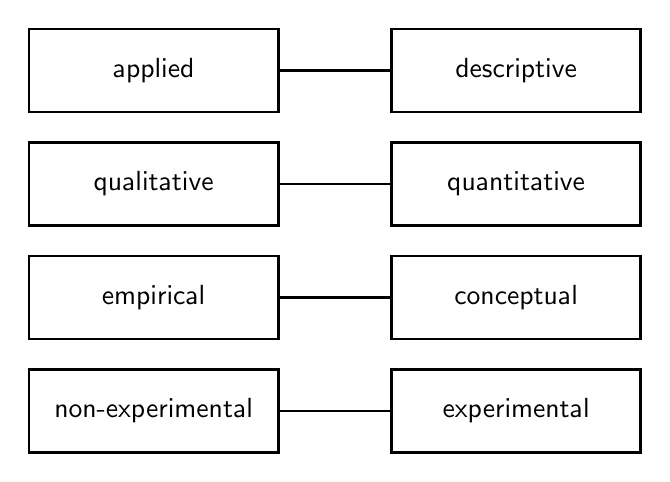
\begin{tikzpicture}
    % Styles
        \usetikzlibrary{shapes,arrows,positioning}
        \tikzstyle{block} = [rectangle, draw, fill=white, text centered, minimum height=3em, minimum width = 9em, line width = 0.1em]
        \tikzstyle{heading} = [fill=white, text centered, minimum height=3em, minimum width = 9em]
        \tikzstyle{line} = [draw, line width=0.1em]
    % left column
        \node [block] (descriptive) {\sffamily{descriptive}};
        \node [block, below = 1em of descriptive] (quantitative) {\sffamily{quantitative}}; 
        \node [block, below = 1em of quantitative] (conceptual) {\sffamily{conceptual}};
        \node [block, below = 1em of conceptual] (experimental) {\sffamily{experimental}};
    % right column
        \node [block, left = 4em  of descriptive] (applied) {\sffamily{applied}};
        \node [block, below = 1em of applied] (qualitative) {\sffamily{qualitative}};
        \node [block, below = 1em of qualitative] (empirical) {\sffamily{empirical}};
        \node [block, below = 1em of empirical] (non-experimental) {\sffamily{non-experimental}};
    % Draw edges
        \path [line] (descriptive) -- (applied);
        \path [line] (quantitative) -- (qualitative);
        \path [line] (experimental) -- (non-experimental);
        \path [line] (conceptual) -- (empirical);
    \end{tikzpicture}
    }
    \caption{Type of research according to \citet{Kumar2008}}
    \label{bodzer-lazaro:fig:1}
\end{figure}

\citet{Williams2002} also make a clear distinction between conceptual (theoretical) research and empirical research, and according to \citet{Borja2009} every research project includes three fundamental phases: conceptual, empirical and interpretative which in the opinion of \citet[102]{Halverson2009} correspond to other ``particular components of vital importance: the research question, research design and assessment of research quality''.

Independently of the classification of research, what is truly important is to be aware of the distinction between two fundamental concepts: \textit{research methods} and \textit{methodology}. The first term (research methods) refers to the techniques and strategies adopted by a researcher while the second term (methodology) represents ``a way to systematically solve the research problems'' \citep[5]{Kumar2008}.

For this paper, it is the empirical phase (or research design) that is of interest to us, as it represents the stage in which the methodological grounds are defined \citep[62]{Borja2009} and the researchers are involved in a continuous meta-level of awareness and decision-making \citep[80]{Halverson2009} while modelling their research methods. In what follows, the different research methods used when researching in the field of public service \isi{interpreting} in specific contexts will be described and illustrated using several examples of studies carried out by the authors in the last five years.

\section{Characteristics of the research carried out in specific contexts}

Analyzing different aspects of the process of \isi{interpreting} or of the interpreter´s role in situations in which the person who does not understand and speak the language of the host country is under a particular pressure or undergoing any kind of traumatic situation turns out to be a very challenging experience and, at the same time, it can pose a risk to the research as the methodology of data collection might have to be adapted to comply with both ethical and sensitive issues. 

One of the first steps that any researcher has to undertake in the incipient phase of gathering data is applying for an official permission. In order to do so, it is necessary to write a formal letter with a brief summary of the project and the kind of information needed as well as an outline of the method or methods to be used. A reply to an official request for permission to be given access to information by a public institution is usually not issued immediately, but can take up to several weeks or even months as sometimes special committees must be formed for this purpose. 

However, an official permission from the institution where the research will be carried out is usually not sufficient, as it is also necessary to count on the acceptance of each and every patient, victim, client, offender, etc. Sometimes, in spite of the official permission from the institution, it is also necessary to obtain consent from the individual employees whose talk will be object of study, as well as from the interpreters, being they employed by the institution or hired by the patient\slash victim\slash client\slash offender.

As it has been mentioned before, many of the settings where public service \isi{interpreting} is performed are tense situations, as one of the interactants (patient\slash victim\slash client\slash offender) is using a public service driven by a personal need or circumstance (a \isi{gender-based violence} victim making a complaint at a police station, a patient who has just had a car crash and is in hospital, a person who finds herself in prison after being charged with theft, etc.) Both the immediacy of the encounters and the personal situation of the speakers make these interactions mediated by an interpreter extremely difficult to research.

Some of the general characteristics of such communications that take place in specific contexts and which will be analyzed for the purpose of our research are outlined below:

\begin{itemize}
\item They take place within an institutional setting.
\item The parties do not share the same language.
\item The presence of an interpreter is needed in order to enable communication.
\item The relationship between the two parties is asymmetrical (both from a linguistic --one party speaks the official language of the country where the encounter takes place and the other one speaks a foreign language- and an educational perspective).
\end{itemize}

All of these characteristics are found in most public service \isi{interpreting} encounters, but, apart from them, there are also others that are more specific to the contexts that will be taken into account for our research:

\begin{itemize}
\item Formal language uttered by service providers.
\end{itemize}
\begin{itemize}
\item Informal language (free narration of the acts, symptoms) uttered by users of public services.
\item Strict institutional protocols.
\item Anonymity and confidentiality are crucial.
\item Different professionals who assist the user (policemen, psychologists, social workers, lawyers, judges, forensic doctors,  nurses, general practitioners, clerks, trainers, etc.)
\end{itemize}

In what follows, different research methods used in projects where members of the Group FITISPos-UAH took part will be presented. All of these projects have in common that they dealt with specific contexts within public service \isi{interpreting}. One of them is a Ph.D. dissertation on \isi{interpreting} in \isi{gender-based violence} trials \citep{Bodzer2014}, which combines interviews, questionnaires, and observation guides.\footnote{Anca Bodzer was awarded a Ph.D. Fellowship by the University of Alcalá for 4 years (from 2010--2014).} Also within the field of \isi{gender-based violence} is the project \textit{Speak Out For Support (SOS-VICS)} (2012--14),\footnote{\url{http://cuautla.uvigo.es/sos-vics/}} aiming at facilitating efficient communications between women who are non-native speakers and victims of gender-based crimes, and the agents who intervene in such acts of communication through well trained interpreters, which was funded by the Directorate-General of Justice of the European Commission. The following two projects were developed in the healthcare setting and included the emergency departments of three different hospitals. The project \textit{Intercultural Mediation for the Healthcare Assistance to Migrant Population: Analysis of Communicative Problems and Suggestions for Training} (2004--07) was funded by the \ili{Spanish} Ministry of Science and Education and aimed at analyzing the quality of communication between clinical staff and foreign patients, at a time when \isi{interpreting} or \isi{mediation} services were not available in hospitals or healthcare centers. Some years later, the project \textit{InterMed} (2012--15), funded by the \ili{Spanish} Ministry of Economy and Competitiveness, set out to \isi{monitor} healthcare mediators in order to assess the quality of mediated healthcare encounters and to establish best practice. The last of the projects involved is \textit{Interpreting and Translation in Penitentiaries} (2013--14), which was funded by the University of Alcalá under the supervision of the \ili{Spanish} Ministry of Economy and Competitiveness and consists of a pilot project aiming at analyzing communicative problems of female inmates in a particular prison located in the vicinity of our university.

\section{Empirical research methods and instruments adopted for specific fields}

Most of the research which has been or is being carried out in the field of public service \isi{interpreting} is designed with the purpose of testing a hypothesis or to describe and analyze the \textit{status-quo} of the profession or other issues related to it (ethics, role of the interpreter, etc.). In order to achieve this, both quantitative and qualitative methods can be used. Each one of methods follows particular objectives, has certain advantages and poses specific problems. For most of research projects, particularly for our descriptive projects, a combination of qualitative and quantitative methods is desired. Several authors, such as \citet{Krolokke2006}, suggest the need of using several research methods which are deliberately recombined. \citet{Creswell2011} offer a convergent parallel design model, which is a data \isi{triangulation} model which implies the parallel application of at least two methods in order to reach the \isi{triangulation} \citep{Denzin1989} or the crosschecking \citep{Douglas1976} of the results of the research or, in Morse's words (\citeyear{Morse1991}: 122), ``to obtain different but complementary data on the same topic''. 

Based on Kumar's \citeyearpar{Kumar2008} \textit{quantitative} versus \textit{qualitative} type of research,\linebreak throughout the following paragraphs we will describe some methods used in our research on \isi{interpreting} in specific contexts and which are also summarized in the figure below:

\begin{figure}
    \resizebox{\textwidth}{!}{
    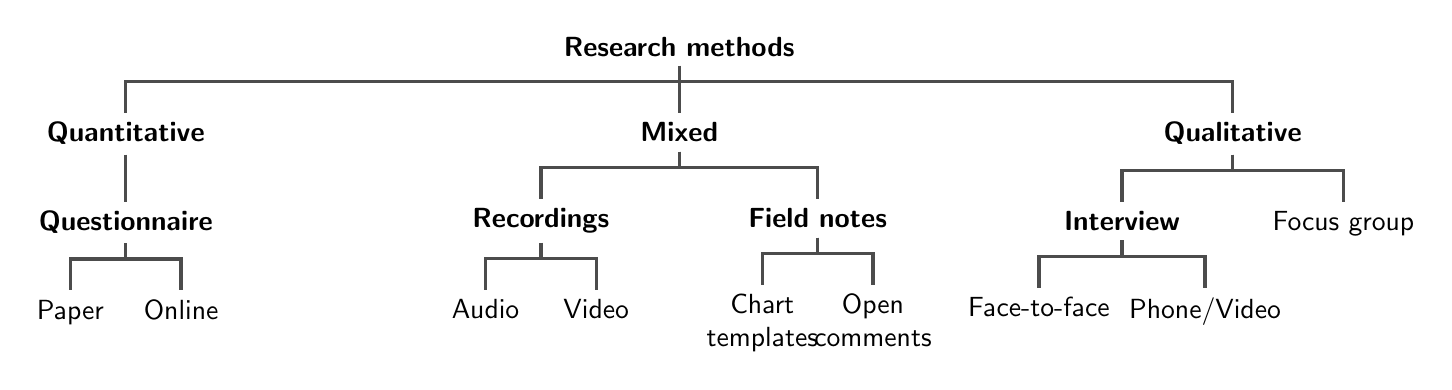
\begin{tikzpicture}[
        level distance=1.7em, 
        edge from parent/.style={very thick,draw=black!70},
        edge from parent path={(\tikzparentnode.south) -- ++(0,-0.2cm) -|(\tikzchildnode.north)},
        growth parent anchor = south, 
        sibling distance = 20em
    ]
    %\usetikzlibrary{positioning,shadows,arrows,trees}

    \tikzstyle{branch} = [ 
        anchor = north, 
        align = center,
        font = \bfseries\sffamily
    ]
    \tikzstyle{leaf} = [
        anchor=north, 
        align=center,
        font = \sffamily
    ]

    \node [branch] {Research methods}
        child {[sibling distance = 0em] node [branch] {Quantitative}
            child {[sibling distance = 4em] node [branch] {Questionnaire}
                child { node [leaf] {Paper}}
                child { node [leaf] {Online}}
            }
        }           
        child {[sibling distance = 10em] node [branch] {Mixed}
            child {[sibling distance = 4em] node [branch] {Recordings}
                child { node [leaf] {Audio}}
                child { node [leaf] {Video}}
            }
            child {[sibling distance = 4em] node [branch] {Field notes}
                child { node [leaf] {Chart \\templates}}
                child { node [leaf] {Open\\ comments}}
            }           
        }
        child {[sibling distance = 8em] node [branch] {Qualitative}
            child {[sibling distance = 6em] node [branch] {Interview}
                child {node [leaf] {Face-to-face}}
                child {node [leaf] {Phone/Video}}
            } 
            child {node [leaf] {Focus group}}
        };
    \end{tikzpicture}
    }
    \caption{Research methods in interpreting specific settings}
    \label{bodzer-lazaro:fig:2}
\end{figure}

\subsection{Quantitative methods} 

Quantitative research is concerned with the measurement of quantity, that is, the relationship among quantifiable variables. One of the most frequently utilized methods consists of using questionnaires. Through this method, researchers try to determine the strength or importance of the correlation between variables and to establish to which degree the results obtained from a sample are objective and general and can be applied to its original population. After this, further analysis aims at explaining the results, which means describing why things happen or do not happen in a particular way. 

\subsubsection{Questionnaire}

Questionnaires are a communication instrument used between the researcher and the group of interest for the investigation. The design of a questionnaire may vary from one research project to another both in length as in form but all of them have some characteristics in common: (1) a brief description of the study including some recommendations on how to complete it, the approximate time needed and the deadline, (2) some initial questions that are geared towards gathering socio-demographic data of the respondents (sex and age) (3) even though they are anonymous. Questions must be clear and specific and questionnaires must be piloted in order to assess their efficacy. Questionnaires can be administered in different ways: in person or remotely, either by sending them to the target population in an envelope and providing at the same time a pre-paid return envelope \citep{Ortega2011} so that the participants can send it back to the researcher by postal service or to be filled in online through the use of specific questionnaire design tools \citep{Bodzer2014}.

Apart from these initial questions designed to profile the respondents, questionnaires may include closed or open questions or a mixture of both. Closed questions can be single or multiple choice questions. Some of the most popular measurements methods used are \citep{Oppenheim2000, Gillham2008}: 

\begin{description}
\item[Likert scale] used to measure attitudes generally expressed in terms of agreement or disagreement although it also allows for measuring a certain degree of neutrality and also the experience of the subject, for example, when questioned about the frequency with which occurrence of a particular fact occurs. The most common form of the Likert scale goes from 1 to 5 (it is symmetrical), but longer scales may also be found, which can be either open (eg. Rate your experience from 1 to 10, 1 being ``very bad'' and 10 ``very good''), or semantically expressed (eg. 1 meaning ``always'', 2 meaning ``often'', 3 meaning ``sometimes''\ldots )
\item[Delphi method] is a method designed for experts which is applied in a repetitive manner since it is used as a prediction tool. The phases of a Delphi questionnaire are represented in \figref{bodzer-lazaro:fig:3}:
\end{description}

\begin{figure}
    \resizebox{.85\textwidth}{!}{
    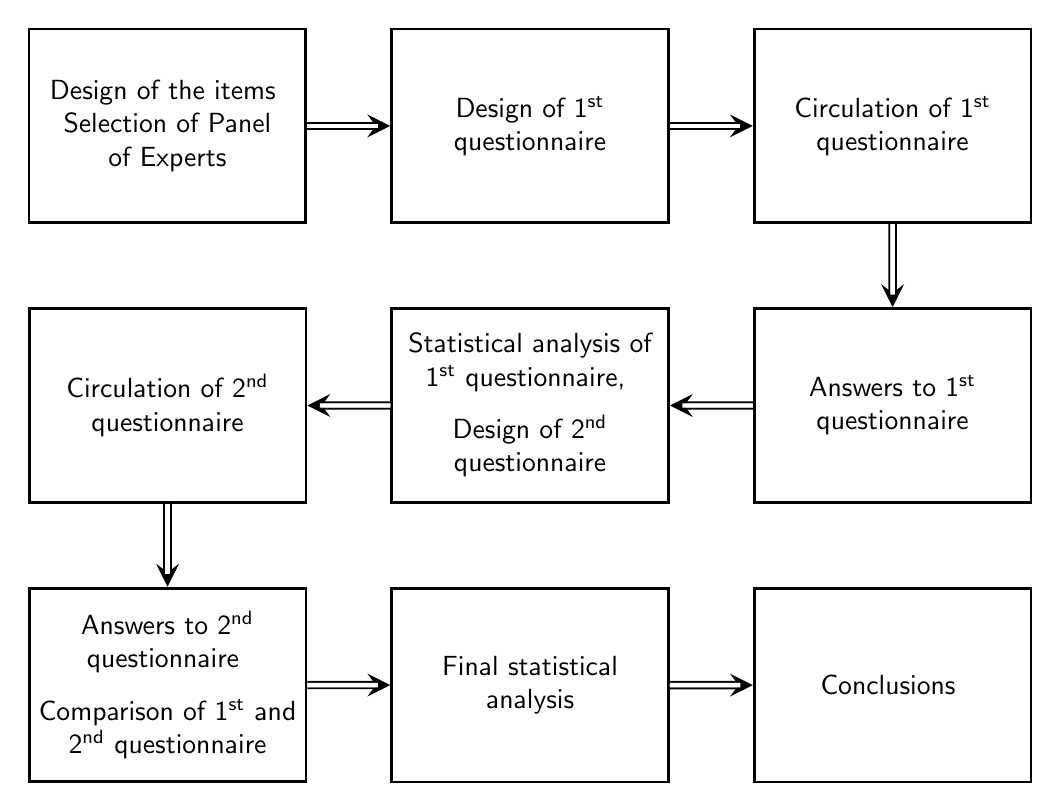
\begin{tikzpicture}[scale=0.6]
    \usetikzlibrary{shapes,arrows,positioning, decorations.markings}
    % Define Styles
        \tikzstyle{block} = [
            rectangle, 
            draw, 
            fill=white, 
            align = center,
            minimum height=7em, 
            minimum width = 10em, 
            line width = 0.1em,
            font = \sffamily
        ]
        \tikzstyle{line} = [
            draw,
            thick, 
            decoration={
                markings,
                mark = at position 1 with {\arrow[scale=2]{stealth}}
            },
            double distance = 1.4pt, 
            shorten >= 5.5pt,
            preaction = {decorate},
            postaction = {
                draw,
                line width=1.6pt,
                white,
                shorten >= 4.5pt
            }
        ]
    % Place nodes
        \node [block] (1) {%
            Design of the items \vspace{0.5em} \\
            Selection of Panel \\ 
            of Experts
        };
        \node [block, right = 3em of 1] (2) {%
            Design of 1\textsuperscript{st} \\
            questionnaire 
        };
        \node [block, right = 3em of 2] (3) {
            Circulation of 1\textsuperscript{st} \\
            questionnaire
        };
        \node [block, below = 3em of 3] (4) {
            Answers to 1\textsuperscript{st} \\
            questionnaire
        };
        \node [block, left = 3em of 4] (5) {
            Statistical analysis of \\
            1\textsuperscript{st} questionnaire, \vspace{0.5em} \\
            Design of 2\textsuperscript{nd} \\
            questionnaire
        };
        \node [block, left = 3em of 5] (6) {
            Circulation of 2\textsuperscript{nd} \\
            questionnaire
        };
        \node [block, below = 3em of 6] (7) {
            Answers to 2\textsuperscript{nd} \\ 
            questionnaire \vspace{0.5em} \\
            Comparison of 1\textsuperscript{st} and \\
            2\textsuperscript{nd} questionnaire
        };
        \node [block, right = 3em of 7] (8) {
            Final statistical \\
            analysis
        };
        \node [block, right = 3em of 8] (9) {
            Conclusions
        };
    % Draw edges
        \path [line] (1) -- (2);
        \path [line] (2) -- (3);
        \path [line] (3) -- (4);
        \path [line] (4) -- (5);
        \path [line] (5) -- (6);
        \path [line] (6) -- (7);
        \path [line] (7) -- (8);
        \path [line] (8) -- (9);
    \end{tikzpicture}
    }
    \caption{Phases of a Delphi questionnaire}
    \label{bodzer-lazaro:fig:3}
\end{figure}

As for the current design of questionnaires, it is more common to use specific electronic tools rather than to adopt the classical form of completing questionnaires on paper. Nevertheless, the option chosen for the design of any questionnaire will directly influence its circulation and, if necessary, the possibility of translating it into other languages should be considered in case an extended sample is needed.

The Internet and new technologies are of great help both with regard to the design of questionnaires but especially with respect to their distribution, storage of information and even analysis of data. Even though there are a lot of free questionnaire design tools available on the Internet, it is very important to be aware of the fact that they do not offer any guarantee and data may be lost without the possibility of recovering it. For this reason, it is strongly recommended to choose a specialized tool and sign up for a paid account. 

Finally, the researcher may consider the option of compensating the respondents for their time and collaboration by giving them the opportunity to leave an e-mail address if they are interested in receiving a summary of data analysis gathered with their help. If this kind of agreement is entered into by the researcher, it must be fulfilled once the data has been analyzed. 

Questionnaires were used for all of the aforementioned projects, either to measure opinions about the quality of communication or to survey personal experiences regarding how communication was carried out. They were usually distributed among all the people involved in the communication process, that is patients\slash clients\slash victims\slash offenders, public service providers, and interpreters or mediators. Two different experiences will now be described: the questionnaires passed on to interpreters by Anca Bodzer as part of her Ph.D. research because of the technical difficulties which arose in the process, and the Delphi questionnaire distributed amongst interpreters with experience in \isi{gender-based violence} contexts as part of the SOS-VICS project. 

  For the Ph.D. dissertation there were five different questionnaires designed as they were addressed to different groups of respondents: interpreters, lawyers, social workers and psychologists and finally non-\ili{Spanish} speaking victims. The first questionnaire designed and piloted was the one directed to the interpreters. It was made up of two parts: the first one included questions that could help establish the profile of the interpreters (sex, age, studies, motivation to be interpreters, etc.) and the second part was more specific as it aimed at gathering information regarding the impact of the gender factor in the process of \isi{interpreting} and analyze the importance of it together with other factors like religion or culture in the specific context of gender violence. For the piloting phase the questionnaire was translated into three languages (\ili{Spanish}, English and \ili{Romanian}) and it was designed using a free specific electronic tool which was previously used for a research at a smaller scale. Unfortunately, because of an internet attack to the page and server of the survey tool the data gathered in two weeks was lost and there was no chance of getting it back. According to this piloting experience it was totally decided that a paid account of a specialized well known tool should be used in during the entire data collection phase in order to guarantee the safety of the data. 

Within the SOS-VICS project, a group of expert translators and interpreters was surveyed in order to find out about the contents that, in their opinion, should be contained in a training program for interpreters and translators working in \isi{gender-based violence} contexts.\footnote{The whole study is published in \citet{DelPozo2013Formacion}} The survey was carried out in two main phases. During the first phase, professionals were openly asked about three aspects: the contents which a training program should cover, the obstacles which prevented them (or other colleagues) from receiving such training, and the most suitable training techniques and strategies to solve this lack of training. Once all the open answers were compiled, a list was elaborated and returned to the professionals. This time, they were asked to rate the items in the list according to their relevance or importance. 

The questions were chosen by a team of five people, all of them researchers involved in the project, but belonging to different fields: translation and \isi{interpreting}, sociology, statistics, and journalism. The respondents were selected by researchers of the nine \ili{Spanish} universities taking part in the project. This made it possible to find experts from all around Spain, thus ensuring the representativeness of the sample. The questionnaire was distributed via email together with the presentation of the project and instructions regarding its completion (including ethical issues related, for example, to the anonymity of the answers).

One of the first obstacles encountered was the difficulty involved in finding respondents with the required profile (translators and interpreters with experience in \isi{gender-based violence} contexts). The second main problem can be attributed exclusively to the nature of the Delphi questionnaire: as it has to be completed in two phases, nearly half of the respondents failed to respond to the questionnaire distributed during the second phase. Two reminders were necessary for each of the phases. Here we can see the aspect of the questionnaire:

Another challenge of this method was to group, reformulate and classify the answers of the respondents for the second phase. A list of 154 items was sent back to the interpreters so that they could rate each of them following a Likert scale (1--5 being 1: ``not important at all'' and 5: ``very important''). This time, a piece of software was used to gather the answers: AdobeFormsCentral. The aim of this phase was to identify the level of importance of each of the items, and also the level of agreement between participants. A third phase had been projected in case the level of agreement had not been high enough after the second phase, but it was ultimately not necessary to carry it out.

\subsection{Qualitative methods} 

Qualitative research focuses on the qualitative phenomenon avoiding quantification and is typically carried out in a natural setting. Adopting a qualitative approach implies the use and collection of a variety of empirical data like participant observation, case studies, personal experiences and interviews, to name just a few \citep[2]{Denzin1994}. Qualitative research tries to identify the deep nature of realities, their system of correlations and their dynamic structure. In the following sections two qualitative methods will be described: interviews and focus groups.

\subsubsection{Interview}

Interviews are particularly useful if one desires to understand opinions or behaviors of a specific group concerning a topic, ``to get the stories behind a participants' experience'' \citep{McNamara1999}. They are conversations based on the researcher's need for data. In other words, it is one of the most frequently used research instrument applied to collect relevant information for the purpose of research. They represent the most common instrument for qualitative research.

Normally interviews are conducted on a face-to-face basis but, with the explosive growth of new technologies, telephone and video interviewing have become more and more common. The only difference between these two kinds of interviews is that the face-to-face interview is synchronous in both time and space while interviews conducted by telephone are asynchronous in terms of space \citep{Opdenakker2006}. Regarding the interviews done via internet there is a debate whether they are asynchronous regarding space or not, as the Internet is considered to be ``no place'' (\citealt{Morse1991} in \citealt{Opdenakker2006}).

As concerns this paper focused on research done in specific fields in which access to information is extremely difficult, the use of technologies such as the phone or the Internet can be of great help during the data collection process. For example, in the special case of gender violence getting to interview victims personally may be impossible for several reasons:

\begin{itemize}
\item The victim does not want to reveal her experience to an unknown person.
\item The victim might feel ashamed in a face-to-face interaction.
\item The presence of an interpreter might be needed and in this case the victim would have to cope with the presence of two unknown persons (researcher and interpreter).
\item The total anonymity (in the majority of the cases) of the victim is crucial for her protection.
\end{itemize}


\subsubsection{Focus group}


Focus groups may be more appropriate than personal interviews for some topics which require further reflection. They represent a discussion with a group of people so that the analysis of data takes place at a level of a group interaction. The participants are chosen because of their expertise, their experiences or their background. Some questions are posed to the participants, who give their individual opinions while listening to the others' opinions, which might serve as an inspiration for the moderator of the focus group to elaborate further opinions.

The main objective of project \textit{InterMed} was to \isi{monitor} teams of healthcare mediators in order to identify and subsequently be able to recommend best practice for a communication mediated by an interpreter\slash intercultural mediator. One of the tasks of mediators working in Spain is usually providing assistance in the elaboration of multilingual materials for a foreign population. Within project \textit{InterMed}, a small scale research project was carried out on health promotion videos addressed to foreign population. The aim was to find out more about their effectiveness and several aspects concerning the levels of adaptation to the audience were studied: linguistic adaptation (dubbing or subtitling), cultural adaptation (communicative styles, proxemics, etc.), and topic adaptation, amongst others. After a first analysis, the study was completed by means of focus groups. Some videos which had been studied by a single researcher were later evaluated by a group of intercultural communication experts and by individuals belonging to the target population (the audience). The evaluation was articulated based on a qualitative and subjective methodology, such as the responsive evaluation model \citep{Stake1976, Abma2005}. This model suggests an evaluation of materials addressed to particular subjects by these same subjects. It is based on qualitative (non-quantifiable) comments and team participation and seeks to capture the singularity of particular situations, allowing for the understanding and evaluation of both processes and results of the health promotion programmes \citep{Gamez2004}.

Although finding experts in intercultural communication and members of medical staff with experience or specialization in interculturality was not a difficult task, finding members of the videos' target community was particularly challenging. \textit{These participants} had to be as close to the target culture as possible, and should not be strongly influenced by the host culture (\ili{Spanish} culture, in this particular study). However, most of the people willing to evaluate the videos, although originally belonging to the target culture, were already very much imbued with the host culture, or were cultural experts themselves, posing the risk that their contributions might be influenced by this fact. This problem was solved when these individuals, instead of participating in the focus group themselves, found other people with the required characteristics within their circles of relatives and acquaintances. 

\subsection{Mixture of qualitative and quantitative research}

Apart from the above mentioned, there is a variety of methods which can be useful both for qualitative and quantitative analysis, as both kinds of data can be compiled and extracted from them. In this article, we would like to mention the analysis of video and audio recordings and the elaboration of observation guides to compile field notes.

\subsubsection{Recordings}

During two of the above mentioned projects, video and audio recordings of medical consultations were compiled. Within the project \textit{Intercultural Mediation for the Healthcare Assistance to Migrant Population: Analysis of Communicative Problems and Suggestions for Training}, carried out from 2004 to 2007, more than 100 recordings were compiled, whereas the researchers of the \textit{InterMed} project, carried out from 2012 to 2015, managed to record around 40 medical consultations. The difference in the number of recordings compiled is striking, taking into account that the duration of both projects was similar and that the methodology which had to be developed for the first project was simply intended to be applied to the second one, without the need of further design. The obstacles encountered in the course of implementing this methodology were manifold, but they were easier to solve in the case of the first project. 

The difficulty revolved around obtaining the informed consent of all the participants in the study and all the speakers whose conversations were to be recorded. First of all, the researcher needs the authorization of the institution in which the conversations are to take place. For the first project, this was obtained after a number of interviews with the managers of the hospital departments and healthcare consultations were the study was carried out. In the case of hospital departments, the head of each department (emergency, pediatrics, and gynecology) was contacted and the project was explained to them. After receiving their verbal authorization, an agreement was signed between the hospital and our university in order to allow for the project to be developed. In turn, the head of the departments held a meeting with their respective department staff to explain the protocol for data compilation. In the case of healthcare centers, several general practitioners were contacted and asked for permission to record their consultations. After they had consented, an agreement form was signed between the healthcare area to which the healthcare centers belonged and our university.

The second step was to obtain permission from the patients to be recorded. A consent form was written by the members of the researcher's team and later translated into several languages (the most common languages of the patients of the area where the study was carried out: English, \ili{French}, \ili{Chinese}, \ili{Arabic}, Polish, \ili{Romanian}, \ili{Russian}), so that foreign patients could read them in their own language. One researcher was present during the consultations and was in charge of explaining the content of the consent form to the patient (objectives of the study, what would be done with the recordings, and how personal data would be processed) and obtained consent from them. It was also the researcher who started and stopped the recorder. The researcher remained silent and as unobtrusive as possible during the consultations.

Apart from the difficulties which arose before the recording phase took place, there were two major problems encountered during the recording phase: the reluctance to participate from both members of staff and patients, and the influence of the presence of the researcher. Some members of staff were concerned about the possibility that their performance might be assessed in terms of quality. On the other hand, patients were afraid that their irregular status of residence in the country would be discovered. Both parties were given explanations about the aims of the study and about the data management process, but reluctance was not completely eliminated.

As the presence of the researcher sometimes influenced the interactions, for example, to the extent that the speakers addressed her and she sometimes became another member in the conversation, some mechanisms were identified to try to minimize this influence. The most effective approach consisted of the members of staff (doctors and nurses) recording the conversations themselves. However, other issues arose: the members of staff forgot to initiate the recorders, or they started it too late, or forgot to stop it, or decided to delete some conversations for a number of different reasons. In the end, this measure was not particularly advantageous, as it did not pose fewer problems.

Some years later, when the \textit{InterMed} project started, a similar methodology was intended to be used. However, the process of obtaining authorization from the institutions was more complicated. Instead of giving their immediate consent, general practitioners and other doctors redirected our request to higher instances. When our proposal reached higher authorities without their prior consent, it was dealt with as an external request and additional documents were requested. We had to solicit an ethics report from the bioethics committee of our university, and our proposal had to be approved by the regional (Madrilean) bioethics committee. Amongst the many documents that we had to present, were the consents forms we planned to give to patients. After the committees' \isi{revision}, the consent forms became long and complicated, and several patients refused to sign them because they did not want to take the time and go to the trouble necessary in order to become informed. 

\subsubsection{Field notes}
\largerpage[-1]
As already mentioned this paper also includes part of the experience of a Ph.D. dissertation based on the analysis of interpretation for non-\ili{Spanish} speaking \isi{gender-based violence} victims during which access to information was decisive for the realization of the study. As access was denied to be present during the interviews with victims or to obtain audioslash video recordings the only approach that allowed for the realization of the research was an ethnographic one based on field notes because, as \citet[12]{Koskinen2008} says, ``the reality of research calls for flexibility, improvising, prioritizing and openness to new opportunities as they arise during the research process''. That is why for this author ``ethnography is a complex methodology which offers a robust and adaptable framework [\ldots ] which allows for using of multiple sources, multiple methods of analysis, and for multiple sites and time-frames'' \citep[6]{Koskinen2008}.

Field notes represent one of the most famous instruments used during the observation period and they may be descriptive or analytical.  Each and every field note should start with information about date, time beginning and time end as well as the location where the observation is carried out. 

Contrary to other approaches that bring the field to the investigator, ethnography and the collection of data based on field notes requires that the researcher go into the field. \citet[3--4]{Schwartzmann1993} states that ``ethnographers go into the field to learn about a culture from the inside out''.

The design and the process of writing field notes is very personal and adapted to each research, and that is why the following information is based on our own experience. Field notes were used along the compilation of data for Anca Bodzer's Ph.D. dissertation and for the project \textit{InterMed}.

The Ph.D. dissertation carried out by Anca Bodzer in the field of \isi{gender-based violence} is based on a corpus of 37 field notes gathered during the daily observation of public judicial trials which took place in specialized courts (\textit{Juzgados de Violencia sobre la Mujer}) in Madrid over the course of seven months. Three of the seven months were in fact a period of accommodation to the field meaning that specialized knowledge about how different courts work, about the role of all the interlocutors (judges, lawyers, prosecutors, witnesses, forensic doctors, social workers and psychologists) and the  different phases of a trial. At the same time, this period helped the researcher test and improve her ability to write down notes based on a very rapid discourse, long sentences and with short or no \isi{pauses} at all, pay attention to what was happening in the room and also to the non-verbal communication. Last, this pre-official three month period of observation was of great help to shape and decide upon the information to be included in the \textit{observation chart template} which would serve as an instrument to collect the same data from all the observed trials. Details like date, timing, type of crime, language(s), gender of interpreter, type of interpretation (simultaneous, consecutive, \textit{chuchotage}, summarized, sight translation) according to each phase of the trial (introduction, victim's\slash accused\slash witness's testimonies, lawyers' reports, etc.) were reflected on the \textit{observation chart template}. A section for open comments was also included with the aim to gather the specific information of each one of the observed trials. This data was extremely helpful to identify the barriers existing in a trial mediated by interpreters and the data was classified following the principles included in the professional code of ethics.

\section{Final remarks}
The purpose of this paper is to promote awareness for the fact that the empirical framework must be shaped or modeled in such a way that it serves to overcome institutional obstacles. At the same time prerequisites such as validity and reliability must be taken into consideration when designing the methods to be used. When conducting research in a specific setting, the use of mixed methods (quantitative and qualitative) represents the only possible way to gather the necessary information. In fact, sometimes adopting typical research instruments like questionnaires and interviews is not enough and other methods must also be taken into consideration and developed. 

Throughout the paper we have presented some relevant methodological information about different typologies of research, while mainly focusing on cases from projects conducted in specific settings in which members of FITISPos-UAH Group took part, placing special emphasis on the difficulties which arose as well as on the methodological solutions that were finally adopted. As nowadays it seems very difficult to obtain access to audio or video recordings from specific settings or to interview persons of interest (gender violence victims) in order to conduct research, our experience showed us that the use of mixed methods and also mixed instruments (observation guides) are of great help.

 
\sloppy
\printbibliography[heading=subbibliography,notkeyword=this]
\end{document}

% 
% {Abma, T. (2005) ``Responsive Evaluation: Its Meaning and Special Contribution to Health Promotion''} {\textit{Evaluation and Program Planning}}{ 28, 279--289}
% 
% Adams, K. and Brace, I. (2006) \textit{Introduction to Market and Social Research}. London
% 
%                 and Philadelphia: Kogan Page
% 
% 
% 
% Angelelli, C. (2004a), \textit{Revisting the Interpreter´s Role,} Amsterdam-Filadelfia: John Benjamins 
% 
% Angelelli, C. (2004b) \textit{Medical Interpreting and Cross Cultural Communication,} Cambridge University Press
% 
% Atkinson, J.M. y Drew, P. (1979) \textit{Order in Court: the Organisation of Verbal Interaction in Judicial Settings}, Londres: Macmillan
% 
% Bischoff, A. (2006) ``Measuring Quality and Patient Satisfaction in Healthcare Communication with Foreign-language Speakers'' in Hertog, E. and  van der ver, B. (eds) \textit{Taking Stock:Rresearch and Methodology in Community Interpreting,} Lingüística Antverpiensa, New Series 5, 177-188
% 
% Bodzer, A. (2014) \textit{Interpretación en los servicios públicos desde la perspectiva de género. Aproximación al caso de las mujeres no hispanohablantes, víctimas de violencia de género}, Universidad de Alcalá, Tesis doctoral, sin publicar
% 
% Borja, A., Garcia Izquierdo, I. and Montalt, V. (2009) ``Research Methodology   in Specialized Genres'' en Mason, Ian (ed.) \textit{Special Issue The Interpreter and Translator Trainer. Training for Doctoral Research}, Manchester: St Jerome
% 
%
% Cambridge, J. (2002) ``Interlocutor roles and the pressure on the interpreter'' in Valero-Garcés, C. and Mancho Barés, G. (eds.) \textit{Traducción e Interpretación en los Servicios Públicos: Nuevas necesidades para nuevas realidades.} Alcalá de Henares: Servicio de Publicaciones de la Universidad de Alcalá, pp. 119-124
% 
%
% 
% Creswell, J.W. and Plano Clark, V.L. (2011) \textit{Designing and Conducting Mixed Methods  Research.} London: Sage
% 
% 
% Davidson, B. (2000) ``The Interpreter as Institutional Gatekeeper: The Social-linguistic Role of Interpreters in \ili{Spanish}-English Medical Discourse'', Journal of Sociolinguistics 4
% 

% 
% Del Pozo Triviño, M., Vaamonde Liste, A., Casado Neira, D., Pérez Freire, S., Vaamonde Paniagua, A., Fernandes del Pozo, D. and Mencía Guinarte, R. (2013b) \textit{Formación especializada en interpretación para víctimas/supervivientes de violencia de género. Informe sobre la encuesta Delphi a intérpretes del proyecto Speak Out for Support (SOS-VICS).} Vigo: Universidad de Vigo
% 
% Denzin, N.K. (1989) \textit{The Research Act}. New Jersey: Prentice Hall
% 
% Denzin, N.K. and Lincoln, Y.S. (eds). (1994) \textit{Handbook of Qualitative Research}, Thousand  Oaks
% 
% Dittmar, N. and Stutterheim, C. (1985) ``On the Discourse of Immigrant Workers: Interethnic Communication and Communication strategies'', en Van Dijk, T.E. (ed.) \textit{Handbook of Discourse Analysis. Discourse Analysis in Society.} London: Academic Press
% 
% Douglas, J.D. (1976) \textit{Investigative Social Research.} Beverly Hills: Sage
% 
% Edwards, A.B. (1995) \textit{The Practice of Court Interpreting}. Amsterdam y Filadelfia: John Benjamins Publishing Company
% 
% 
% Gámez Requena, J.J. and A.C. Márquez Aragonés (2004) `Evaluación de los programas de promoción de la salud para inmigrantes' [Evaluation of health promotion programmes for migrants], in \textit{Index de Enfermería} 13: primavera/verano 2004
% 
% Gentile, A., Ozolins, U., Valilakakos, M. (1996) \textit{Liaison Interpreting}, Melbourne: Melboune  University Press
% 
%
% Gillham, B. (2008) \textit{Developing a Questionnaire} (2\textsuperscript{nd} edition), London, UK, Continuum International Publishin Group Ltd
% 
% Hale, S. (2004) \textit{The Discourse of Court Interpreting Practices of Law, the Witness and the Interpreter,} John Benjamins
% 
% Hale, S. 2007. \textit{Community Interpreting.} Palgrave Macmillan
% 
% Halverson, S.  (2009) Elements of Doctoral Training. The Logic of the Research Process, Research Design, and the Evaluation of Research Quality, en Mason, Ian (ed.) \textit{Special Issue The Interpreter and Translator Trainer. Training for Doctoral Research}, Manchester: St Jerome
% 
%
% 
% Koskinen, Kaisa. 2008. \textit{Translating Institutions. An Ethnographic Study of EU Translation,} Manchester, UK \& Kinderhook: St Jerome
% 
% Krolokke, C. and Sorensen, A. (2006) \textit{Gender Communication: Theories and Analyses.}  London: Sage
% 
% Kumar, R. C. (2008) \textit{Research Methodology}, New Delhi: Nangia
% 
% Lázaro Gutiérrez, R (2012) \textit{La interpretación en el ámbito sanitario. Estudios de la asimetría en consultas médicas,} Editorial Académica Española
% 
% Mikkelson, M (2000) \textit{Introduction to Court Interpreting}, St Jerome Publishing
% 
% McNamara \citet{Carter1999} \textit{General Guidelines for Conducting Interviews}, Authenticity Consulting, LLC.
% 
% Moeketsi, R. (1999) \textit{Discourse in a Multilingual and Multicultural Courtroom: A court Interpreter´s Guide}, JL van Schaik Publishers
% 
% Morse, J. M. (1991) ``Approaches to Qualitative-quantitative Methodological \isi{triangulation}'' en \textit{Nursing Research}, 40, 120-123
% 
% Morris, R. (2010), ``Images of the Court Interpreter. Professional Identity, Role Definition and Self-Image'' en Baer, B. J. (ed.), \textit{Translation and Interpreting Studies}, 5 (1), pp. 20-40
% 
% Opdenakker, R. (2006) ``Advantages and Disadvantages of Four Interview Techniques in Qualitative Research'' in \textit{Forum: Qualitative Social Research,} vol. 7, no. 4, art. 11, available on http://www.qualitative-research.net/index.php/fqs/article/view/175/391 (last consult 27\textsuperscript{th} \citealt{October2014})
% 
% Oppenheim, N (2000) \textit{Questionnaire Design, Interviewing and Attitude Measurement,} (new ed.) London, UK, Continuum International Publishing Group Ltd.
% 
% Ortega Herraéz, J. M. and Foulquié Rubio, A. I. (2005), ``La interpretación en el ámbito jurídico en España: hacía la creación de estructuras estables y profesionales'' en Valero-Garcés, C. (ed.), \textit{Traducción como mediación entre lenguas y culturas/ Translation as Mediation or How to Bridge Linguistic and Cultural Gaps''}, Servicio de Publicaciones de la Universidad de Alcalá, 182-192
% 
% 
% Ortega Herráez, J. M. (2011), \textit{Interpretar para la justicia}, Granada: Comares
% 
% Pöchhacker, F. and Shlesinger, M. (2007) \textit{Healthcare Interpreting. Discourse and Interaction}, John Benjamins
% 
% 
% Raga Gimeno, F. (2006) ``Comunicación intercultural y mediación en el ámbito sanitario'' en Raga Gimeno, F. y Valero Garcés, C. (eds.) ``Retos del siglo XXI en comunicación intercultural: Nuevo mapa lingüístico y cultural de España'', Revista española de lingüística aplicada 1
% 
%
% Schwartzman, Helen. 1993. \textit{Ethnography in Organizations.} Newbury Park: Sage.
% 
% Shlesinger, M and Pöchhacker, F. (2010) \textit{Doing Justice to Court Interpreting,} John Benjamins
% 
%
% Stake, R.E. (1976) \textit{Evaluating Educational Programs: The Need and the Response.} Washington, DC, OECD Publications Center
% 
%
% 
% Pöchhacker, F. (2008) The Turns of Interpreting Studies. In Hansen, Gyden, Chesterman, Andrew, Gerzymisch-Arbogast, Heidrun (eds) \textit{Efforts and Models in Interpreting and Translation Research}, Amsterdam/Philadelphia: John Benjamins, 25-46
% 
% Valero-Garcés (2014) \textit{Health, Communication and Multicultural Communities Topics on Intercultural Communication for Healthcare Professionals,} Cambridge Scholars Publishing
% 
%
% Wadensjö, C. (1998) \textit{Interpreting as Interaction,} London and New York: Longman
% 
% Williams, J. and Chesterman, A. (2002) \textit{The Map: A Beginners Guide to Doing  Research in Translation Studies}, Manchester: St Jerome
% 
